

\chapter{Fejlesztői dokumentáció}
\label{ch:impl}


\section{Megoldandó feladat}
\section{Használt eszközök és környezetek} \label{usedTechnologies}
\subsection{Erlang nyelv}
Az 1980-as évek közepén az Ericsson Számítógép Laboratóriuma azt a feladatot kapta, hogy alkossa meg azt a platformot, ami képes lesz a következő generációs telekommunikációs eszközök kezelésére. Joe Armstrong, Robert Virding, és Mike Williams Bjarne Däcker felügyelete mellett végül megalkották az Erlang porgramozási nyelvet. Ugyan sok már meglévő nyelvet megvizsgáltak, és volt köztük néhány igen ígéretes jelölt, de egyik sem tartalmazta az összes olyan funkciót, ami elvárt volt. A nyelvre hatással volt az ML és Miranda funkcionális nyelvek, valamint olyan konkurens nyelvek, mint az ADA, Chill vagy a Module, illetve a Prolog logikai programozási nyelv. Az első Prolog alapú Erlang virtuális gép prototípus négy év alatt készült el. Végül az Ericsson 1998 decemberében a nyelvet nyílt forrásúvá tette, így bárki számára elérhető lett \cite{erlangBook}.

Az Erlang nyelv a nagy hibatűrő képességének, magas szintű konkurencia támogatásának köszönhetően kedvelt választás elosztott rendszerek fejlesztésében.


\subsection{TypeScirpt}

A TypeScript egy multi-paradigma programozási nyelv, ami lényegében a JavaScirpt nyelvet egészíti ki olyan szintaxis elmekkel, amik segítségével statikus típusozást tudunk elvégezni. TypeScriptben van lehetőségünk szerver- és kliensoldalon is programozni, a különböző keretrendszereknek köszönhetően. A TypeScript kódot futtatás előtt le kell fordítanunk. Itt a fordító elvégzi a szükséges szintaktikus és szemantikus elemzéseket, majd a típus definíciók és megszorítások eltávolítása után előáll a JavaScirpt forrás, amit már a megszokott JavaScript környezetekben futtathatunk \cite{webpageTS} \cite{wikipediaTS}.

Így egy fenntarthatóbb, könyebben kezelhető kódbázist kapunk, illetve a hibákat is előbb kitudjuk szúrni, ha megfelelő típusokat vezetünk be és használunk.

\subsection{Visual Studioc Code API}
A Visual Studio Code egy nyílt forráskódú editor (szekresztő), amit a Microsoft fejleszt és tart karban. A teljes szoftvert olyan elsősorban weben ismert nyelvekkel írták, mint TypeScript, JavaScript, HTML és CSS, ezzel is segítve azt, hogy a legtöbb platformon elérhető legyen \cite{wikipediaVSCODE}.

A fentieken kívül a szerkesztő program rendkívül gazdag fejlesztői dokumentációval és nagyon sok oldalú API-val, vagyis \textit{alkalmazásprogramozási felülettel (Application Programming Interface)} rendelkezik, ami a bővítmények fejlesztését lehetővé teszi. Az editor szinte minden funkcióját tudjunk vezérleni az API-ján keresztül, és ezt a fejlesztést is ez tette lehetővé.

\subsection{WebSocket}
A WebSocket egy számítógépes kommunikációs protokoll, ami teljes duplexitást, azaz kétirányú kommunikációt biztosít egyetlen TCP kapcsolat felett. A tehcnológiát 2011-ben szabványosították és azóta a \textit{Web Hypertext Application Technology Working Group} karbantartásában van, ami egy konzorcium a legnagyobb böngésző gyártokból (\textit{Microsoft, Google, Apple és Mozilla}). \cite{websocketWikipedia}

A portokoll segítségével a kliens és a szerver között mindkét irányban küldhetünk adatot, így nem szükséges a hagyományos kérés-válasz (\textit{request-response}) modellhez alkalmazkodni. Ilyen WebSocket alapú kommunikcáió van a Visualiser bővítmény és a RefactorErl között. 

\subsection{Remote Procedure Calls}
A Remote Procedure Call-nak (RPC), vagyis a távoli eljáráshívásnak a lényege az, hogy egy alkalmazás száméra meghívjon egy függvényt, ami egy távoli számítogépen van implementálva és végre hajtva, úgy mintha lokálisan, helyileg elérhető lenne. A fejlesztőnek megfelelően definiálnia kell a modult és a függvényt, amit végre kíván hajtani a távoli rendszeren, majd a távoli számítógép egy RPC alrendszere ezt a hívást futtatható kóddá alakítja és végrehajta a távoli hívást \cite{distributedSystems}.

A távoli eljáráshívás igen fontos szerepet játszik az elosztott rendszerekben. Az Erlangban egy \lstinline{rpc} modul segíti a fejlesztők munkáját, aminek a megfelelő felparaméterezésével elvégezhetjük a távoli hívást. Ilyen kapcsolatot alakítottam ki a RefactorErl és az Erlang LS node-jai között.



\section{Komponensek}

Az elkészült szoftver komponenseit négy fő részre lehet bontani: Erlang LS-beli illesztő modul, RefactorErl-beli illesztő modul, RefactorErl WebSocket komponense és a Visualiser kiegészítő. Ennek vizualizálásra tekintsük meg a \ref{fig:architecture} ábrát. Az ábrán fellelhető négy komponens nem teljese egészében feleltethető meg az előbb felsoroltakhoz.

A két RefactorErl-beli modult nem különböztettem meg az ábrán, hanem összevönt \textit{RefactorErl}-ként jellemeztem. Továbbá az Erlang LS kliensoldali forrásában nem történt változtatás a dolgozat keretein belül, azonban az architektúra megértése szempontjából fontosnak tartottam jelölni.

Az ábrán felsorolásra kerültek a használt kommunikációs protokollok is, amelyekről a \ref{usedTechnologies} részben olvashatunk bővebben.

\begin{figure}[H]
  \centering
  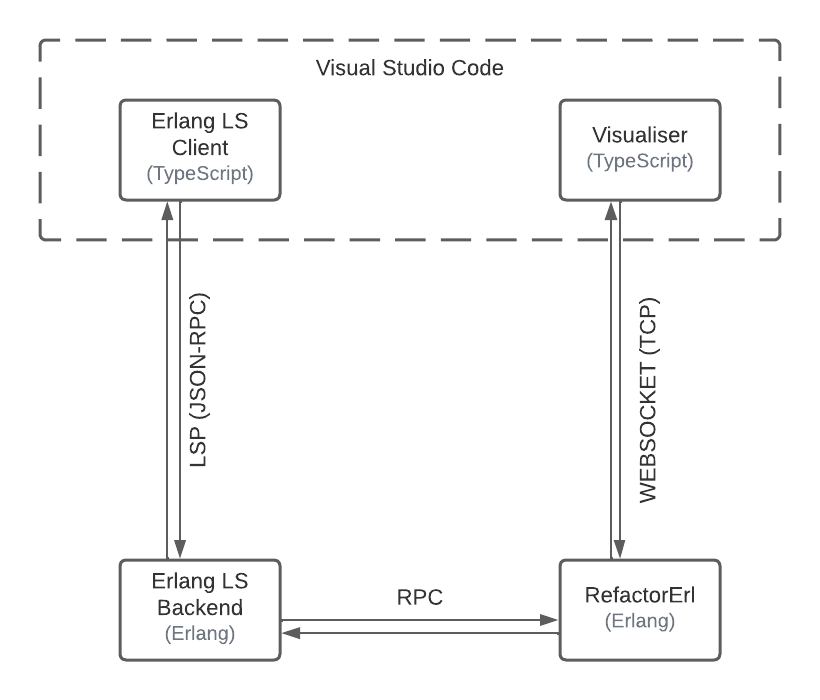
\includegraphics[width=0.8\linewidth]{images/architecture.png}
  \caption{Komponensek viszonya egymáshóz}
  \label{fig:architecture}
\end{figure}

\subsection{Erlang LS-beli illesztő modul}
%\subsubsection{Bevezetés}
Az Erlang LS-ben egy meglehetősen miniális illesztő modul található, mely az üzleti logika jelentős részét a RefactorErlre bízza, hogy a projekt karbantartóinak minél kevesebb idegen kódot kelljen kezelniük. Az Erlang LS (vagy röviden: ELS) néhány helyen tartalmaz kiegészítéseket, most ezeket fogjuk sorra venni.

Az Erlang LS egy aktív projekt, akár havonta többször is jelenhet meg belőle újabb kiadás, ezárt a fejlesztés során a forrást a 21.2-es verziónál rögzítettem, és azt terjesztettem ki a szükgséges illesztő kódokkal

A kommunikáció alapját a \lstinline{els_refactorerl_diagnostics} modul adja, ami nagyban függ a \lstinline{els_refatorerl_utils} modultól. Vizsgáljuk meg közelebbről ezen modulokat.

\subsubsection{\lstinline{els_refactorerl_diagnostics} modul}

\textbf{Erlang Behavior:} Az Erlangban úgynevezett \textit{behaviour} segítségével tudunk álltalános kód részeket kiemelni. Amennyiben több modul is többnyire azonos funkcionalitásokat lát el úgy a generikus, közös részeket behaviourba érdemes kiemelni, a specifikus részt pedig a callback modulban (behaviour megvalósító, kiterjesztő modul) implementálni.

\textbf{Callback függvény:} Az Erlang callback függvénynek nevezünk egy olyan függvényt, aminek az implementálását a \textit{behavior} megköveteli.


Az \lstinline{els_refactorerl_diagnostics} modul az Erlang LS \lstinline{els_diagnostics} behavior-jét egészíti ki. 

A modul az alábbi típusokat definiálja:

\lstset{caption={Típusdefiníciók az \lstinline{els_refactorerl_diagnostics} modulban}, label=src:erlang}
\begin{lstlisting}[language={erlang}]
-type refactorerl_diagnostic_alias() :: atom().
-type refactorerl_diagnostic_result() :: {range(), string()}.
\end{lstlisting}



\begin{itemize}
    \item \lstinline{refactorerl_diagnostic_alias}: szinoníma az \lstinline{atom}-ra
    \item \lstinline{refactorerl_diagnostic_result}: egy pár, aminek első tagja egy \lstinline{range}, ami egy Erlang LS-beli típus, a második tagja pedig egy sztring (szöveges karakterlánc)
\end{itemize}

A modul az alábbi függvényeket definiálja:

\begin{itemize}
    \item \lstinline{-spec is_default() -> boolean().}
        \begin{itemize}
            \item \textbf{Bemenet}: -
            \item \textbf{Kimenet}: logikai típus, hamis
            \item \textbf{Leírás}: \textit{callback függvény}, azt mondja meg, hogy alapértelmezett konfigurációval a diagnosztika fusson-e. Esetünk ez hamis értéket fog visszadni.
        \end{itemize}
     
    \item \lstinline{-spec run(uri()) -> [els_diagnostics:diagnostic()].}
        \begin{itemize}
            \item \textbf{Bemenet}: Uniform Resource Identifier, avagy univerzális erőforrás aznosító, rövide URI. Esetünkben ez egy elérési útvonal lesz, ami az adott elemzendő fájlra mutat.
            \item \textbf{Kimenet}: ELS diagnosztikákat tartalmazó lista
            \item \textbf{Leírás}: \textit{callback függvény}, főbelépési pont a diagnosztikák tekintetében. A diagnosztikák RefactorErl elemzéseiből származik.
        \end{itemize}
    
    \item \lstinline{-spec source() -> binary().}  
        \begin{itemize}
            \item \textbf{Bemenet}: -
            \item \textbf{Kimenet}: A diagnosztika forrása: \textit{RefactorErl}
            \item \textbf{Leírás}:  \textit{callback függvény}, minden diagnosztikának kell lennie egy forrássának, ami a diagnosztika mellett megjelenik.\footnote{Ez sok esetben szokott \textit{Compiler} (azaz fordító) azonosítot tartalmazni, hiszen a fordítóból elég sok diagnosztika származhat. Esetünkben ez \textit{RefactorErl}, hiszen a diagnosztikákat az eszköz állítja elő.} Ez a függvény áthív a \lstinline{els_refactorerl_utils} modulba és onnan tudja meg ezt a konstans információt.\footnote{A későbbi fenntarthatőség és továbbfejlesztés jegyében történt ez a kialakítás}
        \end{itemize}
    
   
    \item \lstinline{-spec enabled_diagnostics() -> [refactorerl_diagnostic_alias()].} 
        \begin{itemize}
            \item \textbf{Bemenet}: -
            \item \textbf{Kimenet}: Az engedélyzett diagnosztika azonosítók listája
            \item \textbf{Leírás}:   A konfigurációs fájl alapján és az \lstinline{els_config} modul segítségével visszatér az engedélyezett 
        \end{itemize}
    
    
    \item \lstinline{-spec make_diagnostics([refactorerl_diagnostic_result()]) -> any().} 
        \begin{itemize}
            \item \textbf{Bemenet}: \lstinline{refactorerl_diagnostic_result}-ból álló lista
            \item \textbf{Kimenet}: ELS-beli \lstinline{diagnostic} típusú lista
            \item \textbf{Leírás}: konvertáló függvény amely átalakítja a input (bemenet) listát, úgy, hogy az ELS megtudja jeleníteni
        \end{itemize}
    \end{itemize}
    
    
\subsubsection{\lstinline{els_refactorerl_utils} modul}
A diagnosztikai modul nagyban támaszkodik a segéd moduljára, a \lstinline{els_refactorerl_utils}, most nézzük meg ezt a modult, hogy milyen függvényeket definiál:

\begin{itemize}
    \item \lstinline'-spec referl_node() -> {ok, atom()} | {error, ErrorReason}. '
        \begin{itemize}
            \item \textbf{Bemenet}: -
            \item \textbf{Kimenet}: 
            \begin{itemize}
                \item \lstinline|{ok, RefactorErlNode}|: a második tagja a párnak tartamazza azt a node-ot amin a RefactorErl fut. Ebben az esetben az RPC alapú kapcsolat a RefactorErl node-al létre jött, használható.
                \item \lstinline|{error, ErrorReason}|: amennyiben a RefactorErl node-al bármi gond van ilyen formában kapjuk a node-ot. Az \lstinline{ErrorReason} a hiba okát tartalmazza. Amennyiben \lstinline{disconnected} az azt jelenti, hogy nem sikerült kapcsolódni a RefactorErl-hez, azonban amint lesz rá lehetőség a rendszer újra fogja próbálni. Ammenyiben \lstinline{disabled} a hiba oka, úgy a node-al a kommunikáció közben valami hiba történt, ami hatására le lett tiltva. Ezt a letiltást csak az Erlang LS újraindításával lehet feloldani. Illetve lehet még \lstinline{other} amennyiben valami olyamsi hiba történt, amire nem készültünk fel korábban.
            \end{itemize}
            \item \textbf{Leírás}: Amikor megnyitunk egy újabb fájlt vagy módosítunk egyet a lemezen, akkor az ELS  lefuttatja (vagy újrafuttatja) a diagnosztikákat, s ekkor intézi az RPC hívást a RefactorErl node-ra. Ehhez ezt a függvényt használja. Amennyiben a kapcsolat még nem jött létre (és nem is lett rossznak ítélve), úgy újra probálkozik annak létrezhozásával.
        \end{itemize}
    
    
    
    \item \lstinline{-spec add(uri()) -> error | ok.}:  Amennyiben az \lstinline{ok} atommal tér vissza, úgy sikeres volt, amennyiben az 
    \lstinline{error} atommal, úgy sikertelen
    \begin{itemize}
            \item \textbf{Bemenet}: globális útvonal
            \item \textbf{Kimenet}: \lstinline{error} atom amennyiben a művelet nem volt sikeres, és \lstinline{ok} atom amennyiben sikeres volt.
            \item \textbf{Leírás}: hozzá adja a paraméterében kapott globális útvonalon elérhető fájlt a RefactorErl adatbázisához, RPC hívással
        \end{itemize}
    
    
    
    
    \item \lstinline{-spec run_diagnostics(list(), atom()) -> list().}:
    \begin{itemize}
            \item \textbf{Bemenet}:  első paraméterében adjuk meg azon diagnosztika azonosítóknak listáját amelyeket szeretnénk futtatni, a második paraméterben, pedig a modult, amire az eredmény halmazt szűkíteni kell
            \item \textbf{Kimenet}: még nyers formátumú diagnosztika
            \item \textbf{Leírás}: RPC hívással lefuttatja a kért diagnosztikákat a kért modulon a RefactorErl node-on
        \end{itemize}
    
    
    
    
    \item \lstinline{-spec notification(string(), number()) -> atom().} 
        \begin{itemize}
            \item \textbf{Bemenet}: Az egy paraméteres verzió esetében információs üzenetet küldhetünk, s magát az üzenet paraméterül adjuk meg. A két paraméteres verzióban a második paraméterrel pontosítani tudjuk azt, hogy milyen típusú üzenetet szeretnénk. Itt használhatjuk 1,2,3 vagy 4 értékekekt, vagy az erre a célra definiált makrókat:
            \begin{itemize}
                \item \lstinline{?MESSAGE_TYPE_ERROR}: hiba típusú értesítés, értéke: 1
                \item \lstinline{?MESSAGE_TYPE_WARNING}: figyelmeztetés típusú értesítés, értéke: 2
                \item \lstinline{?MESSAGE_TYPE_INFO}: információ típusú értesítés, értéke: 3
                \item \lstinline{?MESSAGE_TYPE_LOG}: napló típusú értesítés, értéke: 4
            \end{itemize}   
            \item \textbf{Kimenet}: 
            \item \textbf{Leírás}: egy segéd függvény amivel LSP protokoll feletti értesítéseket tudunk megjeleníteni. 
        \end{itemize}
    
    
    
    \item \lstinline{-spec is_refactorerl(atom()) -> boolean().} 
    \begin{itemize}
            \item \textbf{Bemenet}: Az Erlang node amin feltételezzük, hogy olyan verziójú RefactorErl node fut, ami képes az ELS kommunikálni
            \item \textbf{Kimenet}: igaz érték, amennyiben valóban megfelelő verziójú RefactorErl node fut, különben hamis.
            \item \textbf{Leírás}: A függvény egy RPC hívást intéz a RefactorErl node-jára. Megpróbálja meghívni az ott definiált \lstinline{referl_els:ping/0} függvényt. Amennyiben ez \lstinline|{refactorerl_els, pong}|-al tér vissza, úgy megfelelő verziójú RefactorErl-t futtat a node. Ha bármi mással, melynek oka lehet az, hogy nem megfelelő a verzió, vagy az is, hogy a node-on nem fut az eszköz.
        \end{itemize}
    
    
        
    \item \lstinline|-spec connect_node({validate |\lstinline{| retry, atom()}\lstinline|) -> {error, disconnected} | \lstinline{|} \lstinline| atom().}| 
    \begin{itemize}
            \item \textbf{Bemenet}: Az pár első tagjában a stratégiát határozzuk meg: \lstinline{validate} avagy \lstinline{retry}, a második pedig maga a node nevét adjuk meg
            \item \textbf{Kimenet}: \lstinline|{error, disconnected}|, ha nem jött létre kapcsolat, ha pedig igen, akkor \lstinline|{ok, Node}|, ahol a Node az Erlang node, amit megadtunk.
            \item \textbf{Leírás}: A stratégiát illetően \lstinline{validate} opció esetében a felhasználó tájékoztatva lesz a node állapotáról. Ha korábban már kapcsolat sikeresen felállt, akkor arról, ha pedig most ez nem sikerült akkor arról lesz tájékoztatva. \lstinline{retry} esetén a felhasználó csak akkor lesz tájékoztatva, ha a   
        \end{itemize}
    
    
    
    \item \lstinline{-spec source_name() -> binary().}
    \begin{itemize}
            \item \textbf{Bemenet}: - 
            \item \textbf{Kimenet}: \lstinline{<<"RefactorErl">>.}
            \item \textbf{Leírás}: A diagnosztika modul hívja meg ezt a függvényt. A későbbi bővíthetőség, fenntarthatőség jegyében lett ez ide kiemelve.
        \end{itemize}
    
    
    
    \item \lstinline{-spec variable_orgin(uri(), {number(), number()}) -> error | ok.}
    \begin{itemize}
            \item \textbf{Bemenet}: Első paraméter az útvonal binárosan, a második párban rendre sor és oszlop információ, az adott változóról.
            \item \textbf{Kimenet}: \lstinline{error}, ammenyiben valami hiba történt, \lstinline{ok} ammenyiben mindben rendben.
            \item \textbf{Leírás}: A RefactorErl node felé intézett RPC híváson keresztül kiszámolja egy változó Origin értékét.
        \end{itemize}
    
    
    
    \item \lstinline{-spec variable_reach(uri(), {number(), number()}) -> error | ok.}
    \begin{itemize}
            \item \textbf{Bemenet}: Első paraméter az útvonal binárosan, a második párban rendre sor és oszlop információ, az adott változóról.
            \item \textbf{Kimenet}: \lstinline{error}, ammenyiben valami hiba történt, \lstinline{ok} ammenyiben mindben rendben.
            \item \textbf{Leírás}: A RefactorErl node felé intézett RPC híváson keresztül kiszámolja egy változó Reach értékét, amit Web Socketen keresztül megküldd, a Visualiser bővítmény felé. 
        \end{itemize}
    
    
    
    \item \lstinline{-spec dependency_graph(string(), func | mod) -> error | ok.}
    \begin{itemize}
            \item \textbf{Bemenet}: Az első paraméter a függvény vagy modul nevét tartalmazza rendre \lstinline{<modul_neve>:<függvény_neve>/<aritás>}, illetve \lstinline{<module_neve>} formában.
            \item \textbf{Kimenet}: lstinline{error}, ammenyiben valami hiba történt, \lstinline{ok} ammenyiben mindben rendben.
            \item \textbf{Leírás}: A RefactorErl node felé intézett RPC híváson keresztül kiszámolja egy függvény vagy modul függőségi gráfját, amit Web Socketen keresztül megküldd, a Visualiser bővítmény felé.
        \end{itemize}
    
    
    
    \item \lstinline{-spec dyncall(module(), function(), arity()) -> error | ok.}
    \begin{itemize}
            \item \textbf{Bemenet}: Rendre modul neve, függvény neve és aritása.
            \item \textbf{Kimenet}:  lstinline{error}, ammenyiben valami hiba történt, \lstinline{ok} ammenyiben mindben rendben.
            \item \textbf{Leírás}: Kiszámolja RPC híváson a RefactorErl node-on egy függvénynek a hivatkozásait. Amennyiben a dinamikus analízis el lett végezve, úgy a dinamikus hívásokat is beleteszi.
        \end{itemize}

\end{itemize}




\subsubsection{\lstinline{els_diagnostics} modul módosítása}

A fent leírt kettő modul önmagabán még nem elég. Ahhoz, hogy lefussanak, úgy a \lstinline{els_diagnostics:available_diagnostics/0} függvényét is ki kell még egészíteni. Ez a függvény tartalmazza az elérhető diagnosztikák azonosítóit.

\lstset{caption={Elérhető diagnosztikák módosított verziója}, label=src:erlang}
\begin{lstlisting}[language={erlang}]
-spec available_diagnostics() -> [diagnostic_id()].
available_diagnostics() ->
  [ <<"bound_var_in_pattern">>
  , <<"compiler">>
  , <<"crossref">>
  , <<"dialyzer">>
  , <<"gradualizer">>
  , <<"elvis">>
  , <<"unused_includes">>
  , <<"unused_macros">>
  , <<"unused_record_fields">>
  , <<"refactorerl">>
  ].
 \end{lstlisting}
 
Minden egyes fent felsorolot azonosítóhoz tartozik egy modul, mely implementálj a logikát. A modul neve a következő képpen áll elő: \lstinline{els_<diagnosztika_azonosito>_diagnostics}.

\\

\subsubsection{\lstinline{els_config} modul módosítása}

Ezen kívül ahhoz, hogy a diagnosztikából olvassunk, az \lstinline{els_config} modulba is kellett kiegészítéseket tenni.

\begin{itemize}

    \item A modulban van egy típusdefiníció ami a lehetséges konfigurációs kulcsokat tartalmazza. Ehhez hozzáadtam egy újat: \lstinline{refactorerl}, így most már a bővített típus vázlata:
\lstset{caption={Konfigurációs kulcs, módosított típusdefiníció}, label=src:erlang}
\begin{lstlisting}[language={erlang}]
-type key()   :: apps_dirs
               | apps_paths
               | capabilities
               | diagnostics
               ...
               | refactorerl.
 \end{lstlisting}
 
     \item A modulban van egy másik típusdefiníció ami a konfiguráció állapotának tárolására lesz majd alkalmas. Ehhez hozzáadtam egy kulcsot: \lstinline{refactorerl}, amihez tartozó érték pár vagy a \lstinline{notconfigured} atom, vagy egy \textit{map} típus (kulcs-érték párokat tartalmazó szótár-szerű adatszerkezet, amely hatékony kulcs elérést tesz lehetővé). Ez látható az alábbi kódrészletben:
\lstset{caption={Módosított állapot típus}, label=src:erlang}
\begin{lstlisting}[language={erlang}]
-type state() :: 
#{ apps_dirs        => [path()]
 , apps_paths       => [path()]
 , lenses           => [els_code_lens:lens_id()]
 , diagnostics      => [els_diagnostics:diagnostic_id()]
 ...
 , refactorerl      => map() | 'notconfigured'
 }.
 \end{lstlisting}
 
 \item Következő lépésben megkell keresni a \lstinline{"refactorerl"} kulcsot a konfigurációs fájlban, majd annak értékét beállítani. Ez látható az alábbi kódrészletben:
\lstset{caption={Konfigurációs kulcsmegkeresése, majd beállítása}, label=src:erlang}
\begin{lstlisting}[language={erlang}]
...
RefactorErl = maps:get("refactorerl", Config, notconfigured),
...
ok = set(refactorerl, RefactorErl),
...
 \end{lstlisting}
    
\end{itemize}

Amennyiben a konfigurációs fájlban nem található lilyen kulcs, úgy abban az esetben  \lstinline{notconfigured} lesz beállítva. (Hiszen a \lstinline{maps:get/3} harmadik paramétere azt mondja meg, hogy mi legyen az érték, ha az adott szótárban nincsen olyan kulcs).

Ammeniyben pedig a kulcs sikeresen megtalálható a fájlban úgy, az ELS betölti azt, s rendelkezésnkre adja az eszközölt módosításoknak köszönhetően.

Így már az összes olyan hozzáadott, illetve módosított modult megnéztük, a következő részben a kódakciókat működtető modulokat fogjuk sorra venni. 


\subsubsection{Kódakciók: \lstinline{els_code_action_provider} modul }
A modulban található egy \lstinline{code_action/3} függvény. Ennek kiértékelése kapcsán állnak elő a lehetséges kódakciók. Ezt a függvényt úgy egészítettem ki, hogy az alapértelmezett ELS kódakciókhoz, hozzáfűzi a RefactorErl-nek szánt akciókat az alábbi módon:

\lstset{caption={\lstinline{code_action/3} kibővített verziója}, label=src:erlang}
\begin{lstlisting}[language={erlang}]
-spec code_actions(uri(), range(), code_action_context()) -> [map()].
code_actions(Uri, Range, Context) ->
  #{ <<"diagnostics">> := Diagnostics } = Context,
  Actions0 = [ make_code_action(Uri, D) || D <- Diagnostics],
  Actions = lists:flatten(Actions0),
  RefactorErlActions = referl_action(Uri, Range),
  Actions ++ RefactorErlActions.
\end{lstlisting}

\noindent A RefactorErl eszközhöz szánt kódakciókat a \lstinline{referl_action/2} készíti el. \\
\noindent \lstinline{-spec referl_action(uri(), range()) -> any().}
\begin{itemize}
    \item \textbf{Bemenet:} Az a fájl és tartomány, amire kódakciókat előszeretnénk állítani.
    \item \textbf{Kimenet:} Kódakciókat tartalmazó lista.
    \item \textbf{Leírás:} Ammenyiben a RefactorErl node validálva van, úgy meghívja a \lstinline{variable_action/2}, \lstinline{depgraph_action/2} és \lstinline{dyncall_action/2} függvényeket, hogy kiszámítsák a megfelelő kódakciókat. Amennyiben nincsen ilyen a RefactorErl node validálva, úgy üres listával tér vissza, hisz ez esetben nem akarunk megjeleníteni kódkaciót
\end{itemize}

\noindent \textbf{A kódakciókról}

Összességében a kódakció nem más mint egy szótár adatszerkezet, ami tartalmaz egy \lstinline{title}, \lstinline{kind} és \lstinline{command} kulcsot. A \lstinline{title} lényegében egy bináris szöveg, ami a kódakció szövege, címe lesz. A \lstinline{kind}, vagyis a típusát az LSP protokollban definiáltakból tudjuk megválasztani \footnote{\url{https://microsoft.github.io/language-server-protocol/specifications/lsp/3.17/specification/\#codeActionKind}}. Itt a \lstinline{<<"refactor">>} opciót használtam. A \lstinline{command} esetében pedig a parancs létrehozásához \lstinline{els_command} modul \lstinline{make_command} függvényét használtam. Az alábbiakban látható erre egy példa.

\lstset{caption=Egy példa a kódakcióra, label=src:erlang}\label{codeActionExample}
\begin{lstlisting}[language={erlang}]
CodeAction = #{ title =>  Title
              , kind => <<"refactor">>
              , command => Command }.
\end{lstlisting}

\noindent \textbf{Segdéfüggvények}

\textbf{POI-k az Erlang LS-ben.} Az Erlang LS, a RefactorErlhez hasonlóan elemzi a forráskódot, s a szintaktikai elemeket egy POI struktúrba szervezi. Egy ilyen POI tartalmazza többek között az adott egység kiterjedését és típusát is. A kódakciók kapcsán a POI-k típusára támaszkodtam. Az általam használt típusok:
\begin{itemize}
    \item \lstinline{variable}, vagyis változó;
    \item \lstinline{application}, vagyis függvény alkalmazás, hívás;
    \item \lstinline{function_clause}, vagyis függvény definíciónak egy ága (amennyiben egyetlen ág van, úgy maga a függvény definíció);
    \item \lstinline{module}, vagyis modul. definíció.
    
\end{itemize}

%\begin{itemize}
%    \item 
\noindent \lstinline{-spec variable_action(uri(), range()) -> [map()].}
    \begin{itemize}
        \item \textbf{Bemenet:} Az a fájl és tartomány, amire kódakciókat előszeretnénk állítani.
        \item \textbf{Kimenet:} Kódakciókat tartalmazó lista
        \item \textbf{Leírás:} Az ELS reprezentációjából, kiválogatja változó típusú egységeket, majd a \lstinline{make_variable_action} segítségével elkészíti a rájuk illeszkedő kódakciót.
    \end{itemize}
    
    
    
%    \item 
\noindent \lstinline{-spec make_variable_action(uri(), range(), [poi()]) -> [map()].}
    \begin{itemize}
        \item \textbf{Bemenet:} Az a fájl és tartomány, és a hozzá kapcsolódó POI-k amire kódakciókat előszeretnénk állítani.
        \item \textbf{Kimenet:} Kódakciókat tartalmazó lista
        \item \textbf{Leírás:} Előállítja a kódakció szövegezését és a hozzátartozó parancs hivatkozást.
    \end{itemize}
    
    
    
%    \item 
\noindent  \lstinline{-spec depgraph_action(uri(), range()) -> [map()].}
    \begin{itemize}
        \item \textbf{Bemenet:} Az a fájl és tartomány, amire kódakciókat előszeretnénk állítani.
        \item \textbf{Kimenet:} Kódakciókat tartalmazó lista
        \item \textbf{Leírás:} Az ELS reprezentációjából, kiválogatja függvény hívás és a moduldefiníció típusú egységeket, majd a \lstinline{make_depgraph_action} segítségével elkészíti a rájuk illeszkedő kódakciót.
    \end{itemize}
    
    
    
%    \item 
\noindent  \lstinline{-spec make_depgraph_action(uri(), range(), [poi()]) -> [map()].}
    \begin{itemize}
        \item \textbf{Bemenet:} Az a fájl és tartomány, és a hozzá kapcsolódó POI-k amire kódakciókat előszeretnénk állítani.
        \item \textbf{Kimenet:} Kódakciókat tartalmazó lista
        \item \textbf{Leírás:} Előállítja a kódakció szövegezését és a hozzátartozó parancs hivatkozást.
    \end{itemize}
    
    
    
%    \item 
\noindent \lstinline{-spec dyncall_action(uri(), range()) -> [map()].}
    \begin{itemize}
        \item \textbf{Bemenet:} Az a fájl és tartomány, amire kódakciókat előszeretnénk állítani.
        \item \textbf{Kimenet:} Kódakciókat tartalmazó lista
        \item \textbf{Leírás:} Az ELS reprezentációjából, kiválogatja függvény hívás típusú egységeket, majd a \lstinline{make_dyncall_action} segítségével elkészíti a rájuk illeszkedő kódakciót.
    \end{itemize}
    
  %   \item 
\noindent   \lstinline{-spec make_dyncall_action(uri(), range(), [poi()]) -> [map()].}
    \begin{itemize}
        \item \textbf{Bemenet:} Az a fájl és tartomány, és a hozzá kapcsolódó POI-k amire kódakciókat előszeretnénk állítani.
        \item \textbf{Kimenet:} Kódakciókat tartalmazó lista
        \item \textbf{Leírás:} Előállítja a kódakció szövegezését és a hozzátartozó parancs hivatkozást.
    \end{itemize}
%\end{itemize}


\subsubsection{Kódakciók: \lstinline{els_execute_command_provider} modul }

Eddigiekben láthattuk azt, hogy maga a kódakció hogyan készül el. Egy ilyen kódakciónak része a parancs hivatkozás. Most pedig nézzük meg, hogyan lesz a parancs létrehozva. Egy parancs így épül fel:

\lstset{caption=Egy példa a parancsra, label=src:erlang}
\begin{lstlisting}[language={erlang}]
-type command() :: #{ title     := binary()
                    , command   := command_id()
                    , arguments => [any()]
                    }.
\end{lstlisting}

A parancsnak van címe (\lstinline{title}), azonosítója (\lstinline{command}) és argumentumai (\lstinline{arguments}). Az \lstinline{els_execute_command_provider} modulban az \lstinline{execute_command} függvény definícióját egészítettem ki új ágakkal.

Ezen új ágak:
\begin{itemize}
    \item \lstinline{execute_command(<<"refactorerl-variable-origin">>, Arguments)}
    \item \lstinline{execute_command(<<"refactorerl-variable-reach">>, Arguments)}
    \item \lstinline{execute_command(<<"refactorerl-dependency-graph">>, Arguments)}
    \item \lstinline{execute_command(<<"refactorerl-dyncall">>, Arguments)}
\end{itemize}

Ezen függvény ágak működése roppant egyszerű. Illesztenek a paraméterekre, majd meghívják a megfelelő \lstinline{els_refactorerl_utils} modulbeli függvényt.

Továbbá a modulban megtalálható egy \lstinline{options} nevű függvény, amiben ezen parancsokat regisztrálni kell.

\lstset{caption=\lstinline{els_execute_command_provider:options/0} kibővítése, label=src:erlang}
\begin{lstlisting}[language={erlang}]
-spec options() -> map().
options() ->
  #{ commands => [ els_command:with_prefix(<<"replace-lines">>)
                 , els_command:with_prefix(<<"server-info">>)
                 ...
                 , els_command:with_prefix(<<"refactorerl-variable-origin">>)
                 , els_command:with_prefix(<<"refactorerl-variable-reach">>)
                 , els_command:with_prefix(<<"refactorerl-dependency-graph">>)
                 , els_command:with_prefix(<<"refactorerl-dyncall">>)
                 ] }.
\end{lstlisting}

Az \lstinline{els_command:with_prefix} függvénye előállítja azt a parancsazonosítót mely előtagként tartalmazza egy a környzetre jellemző azonosítót.

\subsubsection{Kommunikáció a többi komponenssel}

Ezen modulok beépülnek, szerves részét képezik az Erlang LS-nek, így természetesen azzal a kapcsolat folyamatos. Ezen kívül a kommunikáció a RefactorErl node-jával RPC kapcsolaton keresztül történik. 

\subsection{RefactorErl-beli LS modul}
\subsubsection{Bevezetés}
\subsubsection{Modul felépítés}

\noindent A modul az alábbi típust definiálja: 
 
\lstset{caption=\lstinline{referl_els} modulbeli típusdefiníció, label=src:erlang}
\begin{lstlisting}[language={erlang}]
-type refactorerl_diagnostic_description() :: {string(), string()}.
\end{lstlisting}
 





\begin{itemize}
    \item \lstinline|-spec refactorerl_diagnostics() -> #{ string() => refactorerl_diagnostic_description() }.|
    \begin{itemize}
        \item \textbf{Bemenet:} -
        \item \textbf{Kimenet:} diagnosztika azonosítók listája
        \item \textbf{Leírás:} visszaadja az elérhető, definiált diagnosztika azonosítók listáját
    \end{itemize}
    
    
    
    \item \lstinline{-spec add(string()) -> error | ok.}
    \begin{itemize}
        \item \textbf{Bemenet:} A hozzáadni kívánt fájl elérési útvonala.
        \item \textbf{Kimenet:} \lstinline{error} vagy \lstinline{ok} az eljárás sikerességétől függően
        \item \textbf{Leírás:} A \lstinline{reflib_ui_router}-en keresztül hozzáad adja az adott fájlt a megadott útvonalon keresztül. A hozzáadás sikerességéről üzenetben kapunk visszajelzést, ennek megfelelően lehet a visszatérése \lstinline{error}, amennyiben valami hiba lépett fel a folyamat közben, \lstinline{ok}, amennyiben sikeres volt a folyamat
    \end{itemize}
    
    
    
    \item \lstinline{-spec run_diagnostic([atom()], module()) -> [referl_els_utils:common_diagnostic()].}
    \begin{itemize}
        \item \textbf{Bemenet:} A diagnosztika azonosítók listája, illetve a modul neve amire futtatni szeretnénk.
        \item \textbf{Kimenet:} Egy köztes diagnosztika leíró lista az Erlang LS és a RefactorErl között.
        \item \textbf{Leírás:} A megadott diagnosztika azonosítóból megkeresi a megfelelő diagnosztika leírót, mely alapján a \lstinline{make_query/2} segédfüggvénnyel elkészíti a lekérdezést. (A segédfüggvénynek még szükséges átadni a modult is amire futtatni szeretnénk) Követekező lépésben a \lstinline{referl_els_utils:query/1} segítségével a lekérdezést lefuttatja, majd a \lstinline{make_diagnostic/2} segítségével előállítja a köztes diagnosztika leírók listáját. Ennek a függvénynek szükséges a \textit{fejléc nélküli} eredmény, melyet a \lstinline{remove_headers} segítségével távolítunk el, illetve az üzenet, amit a diagnosztikával megakarunk jeleníteni.
    \end{itemize}
    
    
    
    \item \lstinline|-spec ping() -> {refactorerl_els, pong}.|
    \begin{itemize}
        \item \textbf{Bemenet:} -
        \item \textbf{Kimenet:} \lstinline|{refactorerl_els, pong}|
        \item \textbf{Leírás:} Arra használatos, hogy egy külső komponens RPC híváson keresztül ellenőrizni tudja, hogy az adott node-on megfelelő RefactorErl fut-e. 
    \end{itemize}
    
    
    \item \lstinline{-spec variable_origin(string(), {number(), number()}) -> ok | error.}
    \begin{itemize}
        \item \textbf{Bemenet:} Elérési útvonal és sor, oszlop páros az adott változó pozíciójának meghatározásához
        \item \textbf{Kimenet:} \lstinline{error} vagy \lstinline{ok} az eljárás sikerességétől függően
        \item \textbf{Leírás:} Az \lstinline{execute_query/5} segítségével kiszámolja a változó Origin értékét és Web Socketen keresztül megküldi a Visualisernek.
    \end{itemize}
    
    
    \item \lstinline|-spec variable_reach(string(), {number(), number()})| \lstinline{ -> ok | error.}
    \begin{itemize}
        \item \textbf{Bemenet:} Elérési útvonal és sor, oszlop páros az adott változó pozíciójának meghatározásához
        \item \textbf{Kimenet:} \lstinline{error} vagy \lstinline{ok} az eljárás sikerességétől függően
        \item \textbf{Leírás:} Az \lstinline{execute_query/5} segítségével kiszámolja a változó Reach értékét és Web Socketen keresztül megküldi a Visualisernek.
    \end{itemize}
    \item \lstinline|-spec execute_query(string(), {number(), number()}, string(), atom(), string())| \lstinline{ -> ok | error.}
    \begin{itemize}
        \item \textbf{Bemenet:}
        \begin{enumerate}
            \item Útvonal
            \item Sor, oszlop páros a pozícióhoz
            \item Lekérdezés (\textit{query})
            \item Küldési azonosító: ezzel az azonosítóval lesz elküldve az eredmény a Visualiser felé
            \item Lebegő információ: ez az információ lesz megjelenítve a Visualiserben, amikor a felhasználó a kurzorát a kijelölés fölé viszi.
        \end{enumerate}
        \item \textbf{Kimenet:} \lstinline{error} vagy \lstinline{ok} az eljárás sikerességétől függően
        \item \textbf{Leírás:} A pozició skalárissá alakítása után a \lstinline{refusr_sq:run/3} segítségével lefuttatja a lekérdezést, majd becsomagolja TODO TODO TODO becsomagolja egy olyan objektumba, amiről itt meg ott na de hol olvashatunk ÉDS és elkuldi a referl vsc websocket:send2  -vel \todo{todo}
    \end{itemize}
    


    \item \lstinline{-spec dynamic_calls(string(), string(), string()) -> ok | error.}
    \begin{itemize}
        \item \textbf{Bemenet:} rendre modul, illetve függvény neve, majd aritása
        \item \textbf{Kimenet:} \lstinline{error} vagy \lstinline{ok} az eljárás sikerességétől függően
        \item \textbf{Leírás:} Előállítja a lekérdezést, majd \lstinline{refusr_sq:run/3} segítségével lefuttatja. \todo{majd becsomagolja és elküldi}. A lekérdezés az alábbi szerkezetű \\ 
        \lstinline{"mods[name=<modul\_neve>].funs[name=<függvény\_neve> and arity=<aritása>].refs"}
    \end{itemize}
    
    
    \item \lstinline{-spec dependency_graph(string(), func | mod) -> ok | error.}
    \begin{itemize}
        \item \textbf{Bemenet:} függvény vagy modul neve, illetve típusa. \lstinline{func} amennyiben függvényre végezzük a lekérdezést, \lstinline{mod} amennyiben modulra.
        \item \textbf{Kimenet:} \lstinline{error} vagy \lstinline{ok} az eljárás sikerességétől függően
        \item \textbf{Leírás:} Elküldi a Web Socketen keresztül a \ref{structOptionsForWs} részletben látható csomagolással a futtatáshoz szükséges paraméterek a Visualisernek, majd annak a feladata lesz lefuttatni. \\
\lstset{caption=Web Socketen keresztül küldött opciók, label=src:erlang}  \label{structOptionsForWs}
\begin{lstlisting}[language={erlang}] 
OptionsForWS = {struct, [
    {"level", "func" | "mod"},
    {"type", "all"},
    {"starting_nodes", [lists:flatten(Name)]},
    {"exclude_otp", false},
    {"exclude", ""},
    {"exclude_lib", ""},
    {"connection", ""},
    {"output_type", ""}
]}
\end{lstlisting}
    \end{itemize}
    
   
\end{itemize}





\subsubsection{Kommunikáció a többi komponenssel}

\todo{TOOD kommunikáció a többi komponenssel}


\subsection{RefactorErl-beli WebSocket komponens}

\subsubsection{Bevezetés}
A következő részekben azon modulokat fogjuk megtekinteni, ami a Web Socketen keresztüli a kommunikációért felelős, legyen szó kérdés-válasz alapú vagy közlés, küldés alapú kommunikációról.

\subsubsection{Adatszerkezetek}
A Web Socketen keresztül bináris formában tudunk adatot küldeni. A könnyű használhatóság érdekében JSON (JavaScipt Object Notion) objektumokat fogunk átküldeni, hiszen ezt a formátumot a TypeScript natívan támogtja, az Erlang pedig a Yaws \lstinline{json2} modulja segítségével használható. Természetesen először szérializálni kell, majd binárissá alakítani.

Legyakrabban JSON szótárakat vagy listákat fogunk átküldeni. A \lstinline{json2:encode/1} függvény az Erlang listákat egyértelműen áttudja alakítani JSON listává, sajnos a szótárak esetében kissé át kell alakítanunk az adatszerkezetünk.

\lstset{caption=Példa szótárak átalakítása, label=src:erlang} \label{mapConvertJson}
\begin{lstlisting}[language={erlang}] 
Struct = {struct, [
            {"key", "value"}, 
            {"key2", ["alpha", "beta"]}
        ]},
Json = json2:encode(Struct),
...
\end{lstlisting}

\lstset{caption=Átalakított példa szótár, label=src:erlang} \label{mapConvertJsonResult}
\begin{lstlisting}[language={erlang}] 
{
    "key": "value",
    "key2": ["alpha","beta"]
}
\end{lstlisting}

Amint a fenti \ref{mapConvertJson} kódrészleten látszodik, ahogyan az adatszerkezetünket szervezni kell, hogy a \ref{mapConvertJsonResult} forrásban lévő eredményt kapjuk. Ez alapján látszik, hogy egy olyan párban kell rendezni, melynek első komponense a \lstinline{struct} atom, a második pedig kulcs-érték párok listája.


\lstset{caption=Egy lekérdezés egyetlen elemének reprezentációja, label=src:erlang} \label{structQueryRes}
\begin{lstlisting}[language={erlang}]
{struct, [
            {"fromPosLn", FromPosL},    % kezdo sor
            {"fromPosCol", FromPosC},   % kezdo oszlop
            {"toPosLn", ToPosL},        % vege sor
            {"toPosCol", ToPosC},       % vege oszlop
            {"name", Name},             % nev infomacio
            {"hoverInfo", HoverInfo},   % lebego informacio
            {"file", File},             % fajl
            {"noPos", false | true}     % tartalmaz-e poziciót?
        ]}
\end{lstlisting}



\subsubsection{\lstinline{referl_vsc} modul}

\noindent \textbf{Néhány fogalom}

\\
\vspace{14pt}

\noindent \textbf{Property} az Erlangban egy propertynek nevezünk egy olyan adatszerkezetet  ami vagy önmagában egy atom vagy kulcs érték pár. Kulcsként legtöbbször atomot választunk, bár ez inkább csak konveció (szokás).

\\
\vspace{14pt}


\noindent \textbf{Property lista} egy olyan lista melynek elemei \textit{property-k}. Gyakran emlegetjük röviden \textbf{proplist}-nek.

\\
\vspace{14pt}

Ez a modul felelős a Yaws webszerver beágyazott módban való elindításáért és felkonfigurálásáért. \cite{zacharyYawsBook}
A modul jelentős részében a \lstinline{referl_web2} modulra épül. Két interfész függvénye van:

\begin{itemize}
    \item \lstinline{start()} vagy \lstinline{start(Props)}: Elindítja az alapértelmezett paraméterekkel a Yaws webszervert. Ezen paramétereket lehet módosítani, amennyiben paraméterül adunk egy property listát.
    \item \lstinline{stop()}: Leállítja a VSC (Visual Studio Code) Visualiser applikációt, és a Yaws webszervert.
\end{itemize}
 
Ez a modul elindítja és leállítja a VSC alkalmazást. Az indításhoz megadható főbb paraméterek:

\begin{itemize}
    \item \lstinline{yaws_port}: A port, amin keresztül Web Socket kommunikálni fog. Ez alapértelmezetten \lstinline{8002} és a Visualiser bővítmény csak ezen a porton képes kommunikálni
    \item \lstinline{yaws_listen}: Az IP\footnote{Internet Protocoll} cím, amin keresztül Web Socket kommunikálni fog. Ez alapértelmezetten \lstinline{127.0.0.1} és a Visualiser bővítmény csak ezen a címen képes kommunikálni
    \item \lstinline{yaws_path}: Az a útvonal, ahonnan a Yaws webszervert indítani szeretnénk. 
\todo{bef}
\end{itemize}

\subsubsection{\lstinline{referl_vsc_sup} modul}

Egy egyszerű felügyelő (\textit{supervisor}) modul, ami újraindít egy gyerek folyamatot, ha azzal bármi baj történik. Ez az úgy nevezett \textit{One for One} (\lstinline{one_for_one}) stratégia. 

\subsubsection{\lstinline{referl_vsc_session} modul}

Egy generikus szerver (\lstinline{genserver}) modul, ami az aktív Web Socketek tárolásért 
felelős. A publikus interfésze lényegébe három fő feladatot lát el: socketetk lekérését, hozzáadását, illetve eltávolítását. Nézzük meg ezeket sorban:

\begin{itemize}
    \item \lstinline{get_websockets/0}: visszaadja az aktívnak vélt socketek azonosítóját.\footnote{Socket a listából csak akkor kerül ki, ha egy küldés művelet nem zárult sikerrel, így elképzelhető, hogy még egyszer küldünk zárt vagy hibás socket-re, de többször nem}
    \item \lstinline{add_websocket/1}: paraméterként adott Socket azonosítót eltárolja
    \item \lstinline{remove_websocket/1}: paraméterként adott Socket azonosítót eltávolítja
\end{itemize}



\subsubsection{\lstinline{referl_vsc_websocket} modul}

Ez a modul felelős a Web Socketen keresztül történő kommunikációért. A publikus interfésze nem kifejezetten bonyolult, azonban a kérések lekezelésére igen sok belső függvény áll rendelkezésre. Nézzük meg először a publikus interfészt:

\noindent \lstinline{handle_open(WSState, State)} \\
\noindent Egy Yaws Callback függvény. Akkor kerül meghívásra, amikor egy új Web Socket akar kapcsolódni. A \lstinline{WSState} tartalmazza a Web Socket azonosítóját, ezt eltároljuk későbbre, amikor közlés alapú küldést szeretnénk végrahajtni (például, mert ELS-ből jött a kérés).

\\
\vspace{14pt}
\noindent \textbf{Publikus interfész}
\\

\noindent \lstinline{handle_message(Message, State)} \\
\noindent Egy Yaws Callback függvény. Akkor kerül meghívásra, amikor egy üzenet érkezik egy Socket felől. A \lstinline{Message} paraméter három kategóriába sorolható, s így a működése is:
\begin{itemize}
    \item \lstinline|{text, <<"client-connected">>}|: egy a klienstől jövő megerősítés a kapcsolat felől
    \item \lstinline|{text, Binary}|: kérések erre az ágra fognak futni, a \lstinline{monitor_handle_request/2} segítségével kezeli le az ide érkező kéréseket
    \item \lstinline|{close, _Status, _Reason}|: Socket lezárásakor érkező kérés.
\end{itemize}
Ez a függvény a végre hajtást a \lstinline{monitor_handle_request/2} segédfüggvény segítségével hajtja végre. Ezt a függvényt fogja elindítani egy külön folyamaton egy ún. Erlang monitor alatt. Ennek a hasznossága az, hogy ha bármi probléma történik a végrehajtás közben, az könyebben lekezelhető, s az összeomlás megakadályozható.
\\


\noindent \lstinline{-spec send(list(), term()) -> error | ok.}\\
\noindent Az első paraméteréül adott eseménytípusra közléssel elküldi, avagy \textit{broadcast}-olja a második paraméteréül adott adatot az összes kapcsolódott Web Socket felé.\\

\noindent \lstinline{-spec broadcast_error(string()) -> error | ok.}\\
\noindent A paraméteréül adott, szöveget az összes kapcsolódott Web Socket felé továbbítja az \lstinline{error} esemény azonosítóval.\\

\noindent \lstinline{-spec broadcast_info(string()) -> error | ok.}\\
\noindent A paraméteréül adott, szöveget az összes kapcsolódott Web Socket felé továbbítja az \lstinline{info} esemény azonosítóval.\\

\\
\vspace{14pt}
\noindent \textbf{Definiált típusok}
\\
\noindent A modul egyetlen szinonímát definiál:
\noindent \lstinline{-type jsonlike() :: term().}


\\
\vspace{14pt}
\noindent \textbf{Belső működése}
\\


\noindent \lstinline{handle_request(Request)}
\begin{itemize}
    \item \textbf{Bemenet:} egy lekérdezés leíró
    \item \textbf{Kimenet:} Yaws válaszobjektum
    \item \textbf{Leírás:} Ez a függvény kezeli le a kéréseket a megfelelő belső függvények hívásával. Vegyük sorra a lehetséges lekérdezés típusokat (\lstinline{requestType}) és a hozzájuk tartozó működést:
    \begin{itemize}
        \item \lstinline{customQueryRequest}: egyedi lekérdezés, meghívja a \lstinline{custom_query_req/1}-t
        
        \item \lstinline{dependencyGraph}: függőségi gráf lekérdezés, meghívja a \lstinline{execute_graph_request/1}-t
        
        \item \lstinline{alive}  egy egyszerű lekérdezés a kliens felől, hogy ellenőrizze a kapcsolat épségét. Egyszerűen \lstinline{"alive"}-t ad válaszul
        
        \item \lstinline{databaseSync}: adatbázis szinkronizációt végez a RefactorErl-n, meghívja \lstinline|execute_simple_ui_request(synchronize)|-t, ami a \lstinline{reflib_ui_router} modulon keresztül elvégi ezt.
        
        \item \lstinline{dynamicAnal}: dinamikus függvényhívás elemzést végez a RefactorErl-n, meghívja \lstinline|execute_simple_ui_request(analy_dyn)|-t, ami \lstinline{reflib_ui_router} modulon keresztül elvégi ezt.
        
        \item \lstinline{dynamicClear}: dinamikus függvényhívás elemzésének eredményét törli a RefactorErl-n, meghívja \lstinline|execute_simple_ui_request(clean_dyn)|-t, ami \lstinline{reflib_ui_router} modulon keresztül elvégi ezt.
        
        \item Amennyiben olyan lekérdezés érkezett, ami nem tartalmaz típus azonosítót vagy olyat tartalmaz, amit nem ismerünk, úgy ezt hibakét jelezzük.
        
    \end{itemize}
\end{itemize} \\



\noindent \lstinline{-spec create_broadcast_event(list(), term()) -> {text, jsonlike()} \lstinline|}.}|
\begin{itemize}
    \item \textbf{Bemenet:} Első paraméter egy esemény azanosító, a második pedig egy olyan adat, amit a \lstinline{json2:encode} függvénye JSON szöveggé tud alakítani
    \item \textbf{Kimenet:} Egy olyan pár, melynek első tagja a \lstinline{text} atom, illetve a második tagja pedig egy JSON szerű szöveg. 
    \item \textbf{Leírás:} A megadott esemény azonosítóval előállítja azt az adatszerkezetet, amivel az adatot áttudjuk küldeni. Ez lesz a pár második tagja. ez az adatszerkezet valahogy így néz ki:
\lstset{caption=Esemény alapú küldés szerkezete, label=src:erlang} \label{structQueryRes}
\begin{lstlisting}[language={erlang}]
{struct, [
    {"event", Event},       % esemeny azonosito
    {"data", Data},         % adat
]}
\end{lstlisting}
\end{itemize} \\

\noindent \lstinline{-spec create_callback_event(undefined | string(), term()) -> ok | error | {text, jsonlike()} \lstinline|}.}|
\begin{itemize}
    \item \textbf{Bemenet:} Első paraméter egy visszaküldési azanosító, a második pedig egy olyan adat, amit a \lstinline{json2:encode} függvénye JSON szöveggé tud alakítani. \lstinline{undefined} is megengedett.
    \item \textbf{Kimenet:} egy olyan pár, melynek első tagja a \lstinline{text} atom, illetve a második tagja pedig egy JSON szerű szöveg, vagy maga az \lstinline{ok} vagy \lstinline{error} atomok
    \item \textbf{Leírás:} Amennyiben a bemenetnél \lstinline{undefined} értéket kapunk, úgy nem, lehet visszaküldési azonosítóval elküldeni, ekkor a hibát szétküldjük az ismert Socketeknek. Ha ez sikerrel zárult, akkor \lstinline{ok} atom, ha nem akkor \lstinline{error} atomot kapunk vissza. \\ \\ Ha visszaküldési azonosítót kapunk, akkor előállítja azt az adatszerkezetet amivel az adatot áttudjuk küldeni. Ez lesz a pár második tagja, míg az első a \lstinline{text} atom lesz. Ez az adatszerkezet valahogy így néz ki:

\lstset{caption=Visszaküldési azonosítós küldés szerkezete, label=src:erlang} \label{structQueryRes}
\begin{lstlisting}[language={erlang}]
{struct, [
    {"callbackId", Event},      % visszakuldesi azonosito
    {"data", Data},             % adat
]}
\end{lstlisting}
\end{itemize} \\

\noindent \lstinline{-spec get(list(), term()) -> term().}
\begin{itemize}
    \item \textbf{Bemenet:} első paramétere egy kulcs, a második egy lekérdezés leíró
    \item \textbf{Kimenet:} bármilyen Erlang term, ami a kulcs alatt van
    \item \textbf{Leírás:} A megadott kulcson található értéket visszadaja a lekérdezés leíróból. Amennyiben a kulcs nincs jelen úgy, \lstinline{undefined}-ot ad vissza.\\ \\ Egy lekérdezés leíró lényegében egy kulcs érték pároból álló lista, ami Web Socketen kersztül érkezik.
\end{itemize} \\

\noindent \lstinline{-spec cbId(term()) -> term().}
\begin{itemize}
    \item \textbf{Bemenet:} Egy lekérdezés leíró
    \item \textbf{Kimenet:} A visszaküldési azonosító, amennyiben a lekérdezés leíróban jelen van. Ha nincs jelen, akkor \lstinline{undefined}
    \item \textbf{Leírás:} Egyszerű kis segédfüggvény, ami visszadja a visszaküldési azonosítót ha jelen van a \lstinline{get/2} segítségével.
\end{itemize} \\

\noindent \lstinline{-spec dot_to_svg(string()) -> {ok, string()} | file_notexists | error | timeout.}
\begin{itemize}
    \item \textbf{Bemenet:} Egy elérési útvonal, ahol a DOT file található
    \item \textbf{Kimenet:} 
    \begin{itemize}
        \item \lstinline|{ok, string()}|: amennyiben sikerrel zárult a művelet, akkor a pár második komponensében lesz az SVG fájl elérési útvonala
        \item \lstinline|file_notexists|: amennyiben a megadott fájl nem létezik
        \item \lstinline|error|: az eljárás közben hibatörtént
    \end{itemize}
    \item \textbf{Leírás:} Az \lstinline{erlang:open_port/2} segítségével egy rendszerhíváson keresztül átalakítja a DOT fájlt SVG fájllá.
\end{itemize} \\


\noindent \lstinline{-spec construct_path(list()) -> list().}
\begin{itemize}
    \item \textbf{Bemenet:} egy fájlnév
    \item \textbf{Kimenet:} egy útvonal
    \item \textbf{Leírás:} a megadott fájlnévhez előállítja az adatkönyvtárbeli útvonalat.
\end{itemize} \\


\noindent \lstinline{custom_query_req(Request)}
\begin{itemize}
    \item \textbf{Bemenet:} egy lekérdezés leíró
    \item \textbf{Kimenet:} egy válasz objektum, amit a Yaws webszerver küld vissza
    \item \textbf{Leírás:} A megadott lekérdezést végrehajtja, majd az eredményt olyan formátumra hozza, hogy a Visualiser komponens könnyen megtudja jeleníteni, illetve csak a szükséges információkat tartalmazza. Az átalakításhoz használt segédfüggvények:
    \begin{itemize}
        \item \lstinline{construct_position_response/8}: lényegében egy pozíciós választ állít elő, ami a \ref{structQueryRes} forrásban mutatott szerkezettel megegyezik
        
        \item \lstinline{position_convert/2}: egy RefactorErl pozíció válaszból és egy lebegő információból a \lstinline{construct_position_response/8} meghívásával pozíciós választ állít elő
        
        \item \lstinline{construct_poslist_response/3}: egy RefactorErl pozíció válasz listából és egy lebegő információból, illetve egy fájl névből a \lstinline{position_convert/2} meghívásával pozíció listás választ állít elő, melynek szerkezete: (lásd \ref{poslistResp} forrás)
        
\lstset{caption=Pozíció listás válasz, label=src:erlang} \label{poslistResp}
\begin{lstlisting}[language={erlang}]
 {struct, [
    {"file", File},         % fajl
    {"items", PosList }.    % pozicio lista
]}.
\end{lstlisting}

    \item \lstinline{construct_eq_response/3}: egy RefactorErl pozíció mentes válasz listából és egy lebegő információból, illetve egy fájl névből a \lstinline{construct_position_response/8} meghívásával pozíció mentes listás választ állít elő, mely esetlben a sor, oszlop információk 0 értéket tartlamzanak, illetve \lstinline{noPos} kulcs alatt igaz érték fog szereplni.
        
        
\end{itemize} \\
    \end{itemize}
    
    
\end{itemize} \\


\noindent \lstinline{-spec get_graph_options(list()) -> list().}
\begin{itemize}
    \item \textbf{Bemenet:} egy \textit{proplist} ami Web Socketen keresztül érkezett és a kulcsai lehetnek: \lstinline{"type", "level", "starting_nodes", "exclude_otp", "exclude", "exclude_lib", "connection", "output_type"}. ezek hasonlóak, mint ahogy Shell-ből paramétereznénk a gráf lekérdezést. \cite{referlWikiDependency}
    \item \textbf{Kimenet:} Egy olyan property lista, ami átadható a gráf lekérdezésnek.
    \item \textbf{Leírás:} A szükséges ellenőrzések és átalakítások után a Web Socketen keresztül érkezett adatszerkezetből a RefactorErl függőségi gráf készítőjének átadható listát állít elő.
\end{itemize} \\



\noindent \lstinline{-spec request_class(list()) -> simple | construct | unknow.}
\begin{itemize}
    \item \textbf{Bemenet:} egy szöveg, ami a lekérdezés típusát tartalmazza
    \item \textbf{Kimenet:} a lekérdezés osztálya, ami lehet \lstinline{simple}, \lstinline{construct} vagy ismeretlen (\lstinline{unknow})
    \item \textbf{Leírás:} egy lekérdezés azonosító alapján megmondja, hogy mely kategóriába sorolható.
    \\ \lstinline{simple} kategória: \lstinline{"databaseSync", "dynamicAnal", "dynamicClear"}
    \\ \lstinline{construct} kategória: \lstinline{"customQueryRequest", "dependencyGraph"}
    \\ \lstinline{unknow} kategória: minden más
\end{itemize} \\


\noindent \lstinline{execute_graph_request(Request)}
\begin{itemize}
    \item \textbf{Bemenet:} egy lekérdezés leíró
    \item \textbf{Kimenet:} Yaws válasz objektum
    \item \textbf{Leírás:} a megadott lekérdezés leíróban található  gráf lekérdezést végrehajtja és a szükséges adatokat visszaküldi. Amennyiben a gráf szöveges ábrázolású, úgy a teljes gráfót átküldi, míg SVG reprezentáció kérése esetén csupán a fájl elérését. Az utóbbi esetben használja a \lstinline{construct_dot_response/1} segédfüggvényt, amely a DOT fájllá alakítás sikerességétől függően előállítja a válasz vagy hibaobjektumot.
\end{itemize} \\


\noindent \lstinline{error_reply(Request)}
\begin{itemize}
    \item \textbf{Bemenet:} egy lekérdezés leíró
    \item \textbf{Kimenet:} Yaws válasz objektum
    \item \textbf{Leírás:} a \lstinline{request_class/1} alapján a megfelelő formátumú hibát fogja küldeni. Ez végső esetben használatos, amikor nem teljesen nyílván való a hiba oka.
\end{itemize} \\




\subsubsection{Kommunikáció a többi komponenssel}

Ez a komponens a RefactorErl szerves részét képzi, így azzal nyílvánvaló módon kommunikál, továbbá Web Socketen keresztül a Visualiser komponenssel.


\subsection{RefactorErl Visualiser kiegészítő}

Mivel az Language Server Protocoll kissé limitált a megjelenítő eszközök tekintetében, ezért nem lehetett minden tervezett RefactorErl funkcionalitást használható módon integrálni az Erlang LS-be. Ezen hiányosság áthidalása érdekében született meg a Visualiser kiegészítő.

\subsubsection{Áttekintés}

\begin{figure}[H]
  \centering
  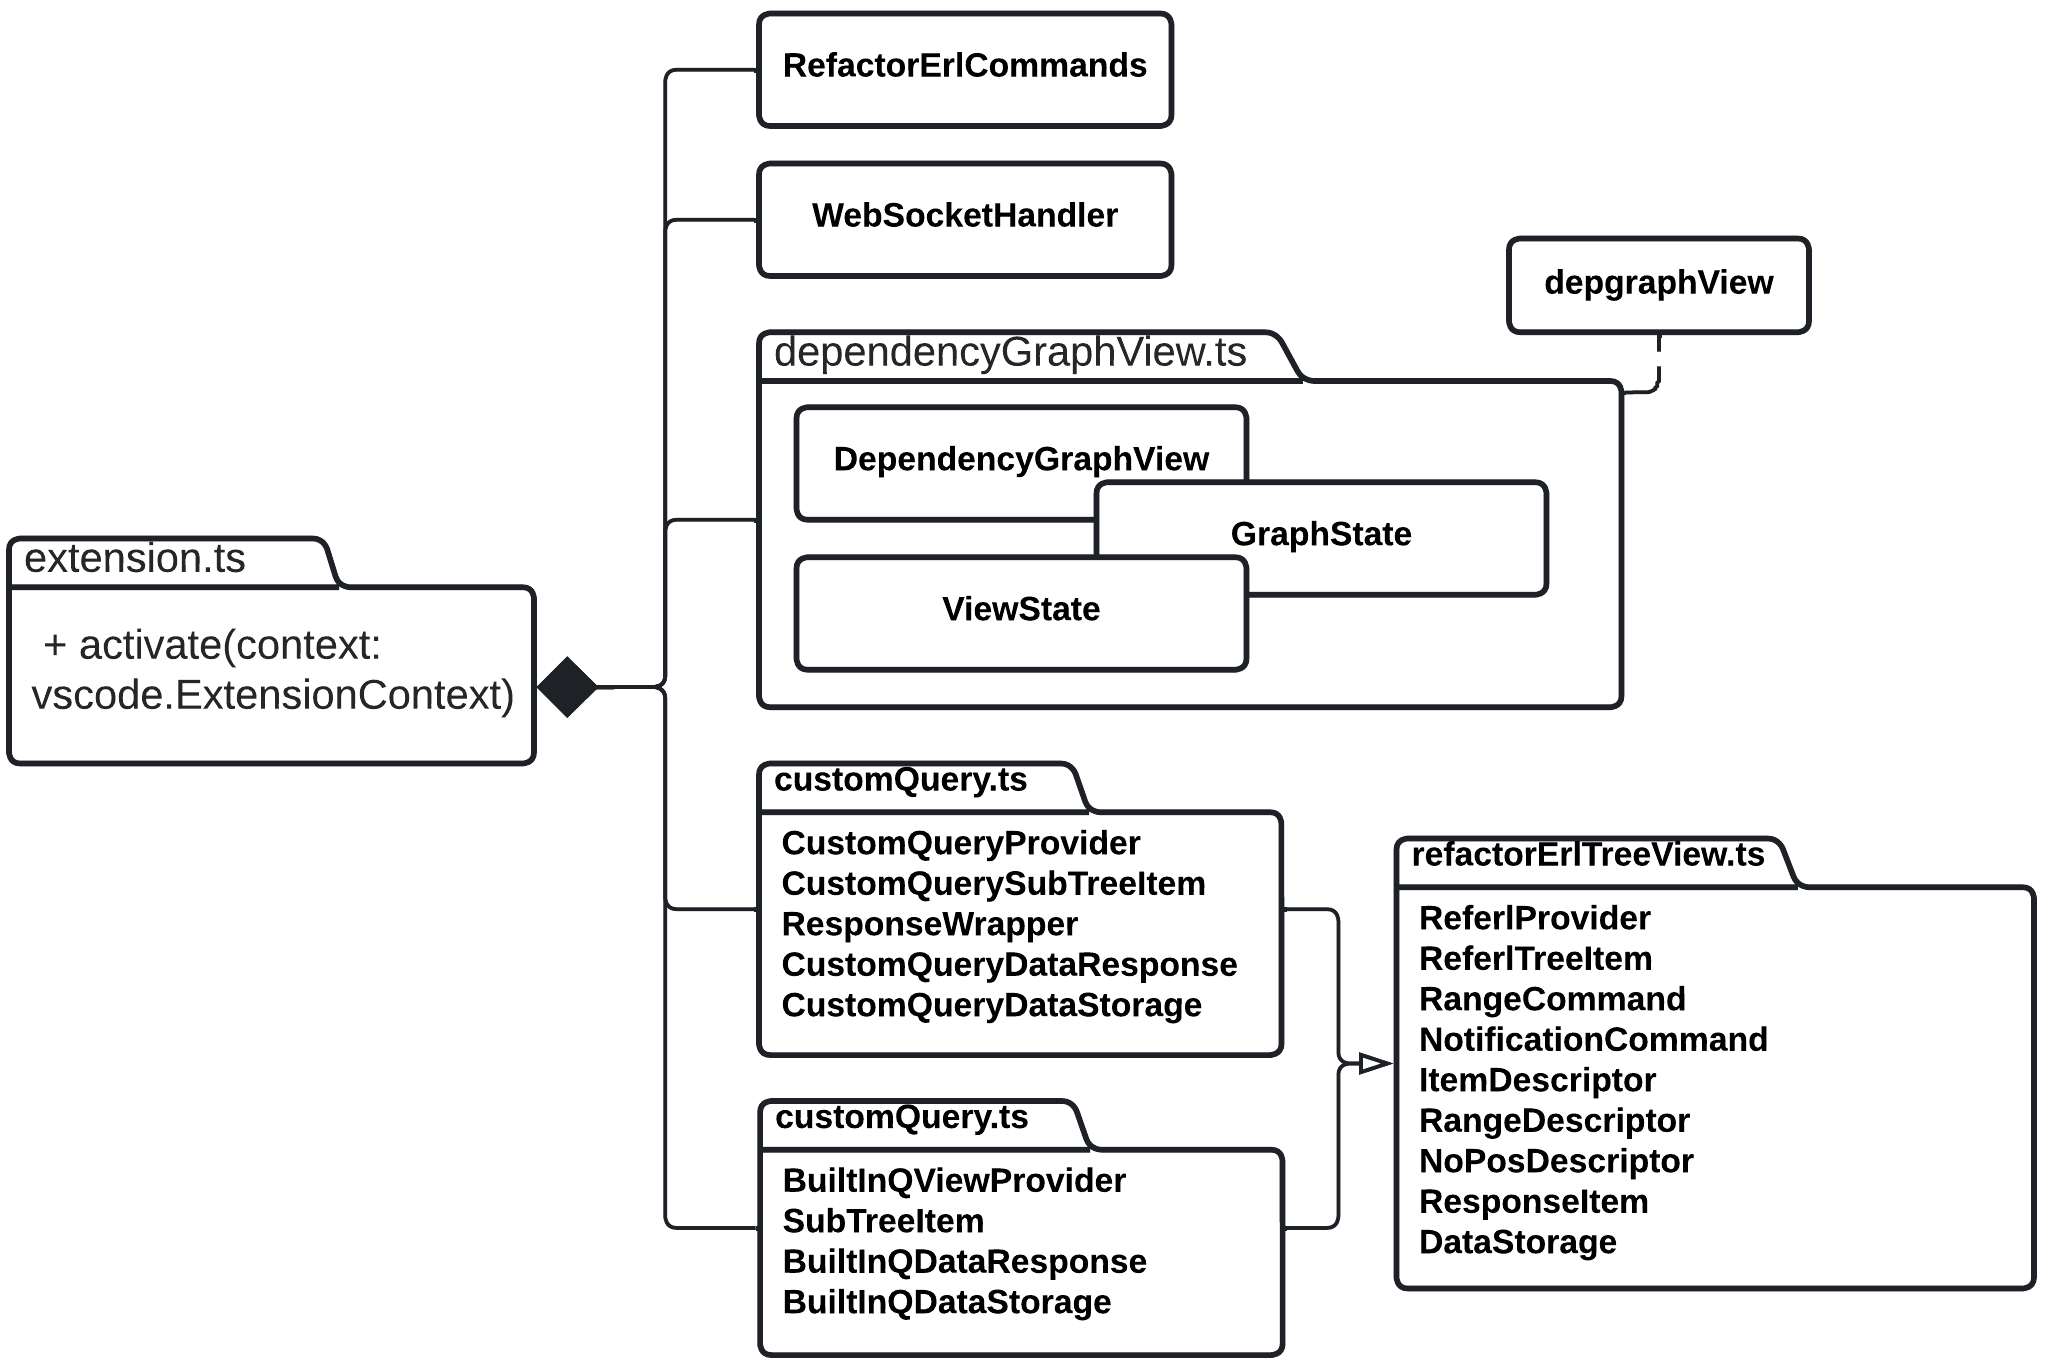
\includegraphics[width=\linewidth]{images/visualiser_arch.png}
  \caption{Visualiser alkomponenseinek viszonya egymáshóz}
  \label{fig:visualiserArch}
\end{figure}

A Visualiser is több alkomponensre bontható fel, mely a \ref{fig:visualiserArch} ábrán látható. Vegyük ezeket sorra, és tekintsük meg működésüket.

\subsubsection{\lstinline{extension.ts}}

Ez fő belépési pontja a kiegészítőnek, mindösszesen egyetlen függvénye van: az \lstinline{activate}, ami paraméteréül a Visual Studio Code kontextusát kapja, majd elkezdi aktíválni a bővítményt a következő lépésekkel:

\begin{enumerate}
    \item Példányosítja a beépített (\lstinline{BuiltInQViewProvider}) és a egyéni lekérdezések (\lstinline{CustomQueryProvider}) megjelenítőit és regisztrálja a szerkesztő számára
    \item Párosítja a Web Socket felől érkező eseményeket a megfelelő eseménykezelőkkel
    \item A Web View-t vagyis a \lstinline{DependencyGraphView}-t is inicializálja
    \item A szükséges parancsokat a \lstinline{RefactorErlCommands} segítségével beállítja
    \item Az egyedi lekérdezésekhez szükséges dialógust inicializálja
\end{enumerate}

\subsubsection{\lstinline{RefactorErlCommands} osztály}

Lényegében egyetlen osztályszintű függvént tartalmaz: \lstinline{setCommandForContext}, aminek paraméteréül a szerkesztő kontextusát kell megadnunk, majd ehhez a kontextushoz beállítja az alábbi parancsokat:

\begin{itemize}
    \item \lstinline{builtinView.goToLocation} és \lstinline{customQuery.goToLocation}: arra használatos, hogy egy \lstinline{RangeDescriptorral} megadott pozícióra ugorjunk
    
    \item \lstinline{customQuery.noPosNotify} ammenyiben nem áll rendelkezésre pozíció ezen parancs segítségével adunk erről a felhasználónak értesítést
    
    \item \lstinline{refactorErl.checkConnection}: ezen parancs segítségével tudjuk a Vezérlőpult (\textit{Dashboard}) felületéről a kapcsolatot ellenőrizni
    
    \item \lstinline{refactorErl.tryAgainConnect}: ezen parancs segítségével tudjuk a Vezérlőpult (\textit{Dashboard}) felületéről a kapcsolódást újrapróbálni
    
    \item \lstinline{refactorErl.dependencyGraph}: ezen parancs segítségével jelenítjük meg függőségi gráf nézetét a \textit{Command Palette}-ről kiadott utasítás alapján
    
    \item \lstinline{refactorErl.databaseSync}:  ezen parancs segítségével tudjuk a Vezérlőpult (\textit{Dashboard}) felületéről az adatbázis szinkronizációját elvégezni
    
    
    \item \lstinline{refactorErl.dynamicAnal}: ezen parancs segítségével tudjuk a Vezérlőpult (\textit{Dashboard}) felületéről az dinamikus függvényhívás elemzését elvégezni
    
    \item \lstinline{refactorErl.dynamicClear}: ezen parancs segítségével tudjuk a Vezérlőpult (\textit{Dashboard}) felületéről az dinamikus függvényhívás elemzésének eredményének törlését elvégezni
    
\end{itemize}


\subsubsection{\lstinline{refactorErlTreeView.ts}}

Ebben a fájlban a \lstinline{ReferlProvider} osztály implementációja és a hozzátartozó segéd típisuok, osztályok és interfészek.

\\
\vspace{14pt}
\textbf{ReferlProvider}
\\

Ez az osztály lényegében egy sablon, absztrakt osztály a beépített és az egyedi lekérdezéseknek. Implementálja a \lstinline{vscode.TreeDataProvider} interfészt. Vizsgáljuk meg a nyílvános részei.

\begin{itemize}
    \item \lstinline{refresh(data: any): void}: ezen függvénynek adhatjuk paraméterül a frissített adatot amit a fa nézetben megszeretnénk jeleníteni
    
    \item \lstinline{static selectTreeItem(rangeDescriptor: RangeDescriptor, decoration: vscode.TextEditorDecorationType, message: string)}: az első paraméterben megadott helyre állítja a szerkesztőt, majd a második paraméteréül kapott dekorációs stílusokat alkalmazza rá, s a harmadik paraméterben kapott üzenet lesz az az üzenet, ami akkor jelenik meg ha a felhasználó a kurzorát fölé viszi
\end{itemize}

\\
\vspace{14pt}
\textbf{ReferlTreeItem}
\\

Ez egy egyszerű fa elem, ami minimálisan a \lstinline{vscode.TreeItem} \footnote{https://code.visualstudio.com/api/references/vscode-api#TreeItem} osztályt bővíti ki. Lényegében egy konstruktora van, amiben rendre megadhatjuk a címet, az alcímet, összecsukási állapotot, a parancsot és az ikonok elérési útját, bár az utóbbi kettő nem kötelező.


\\
\vspace{14pt}
\textbf{ItemDescriptor}
\\

Egy interfész, amely az alábbi adattagok jelenlétét követeli meg:
\begin{itemize}
    \item \lstinline{title}: szöveg
    \item \lstinline{hasRange}: logikai
    \item \lstinline{subtitle}: szöveg
\end{itemize}


\\
\vspace{14pt}
\textbf{RangeCommand}
\\

Ez egy egyszerű fa elem, ami minimálisan a \lstinline{vscode.Command} \footnote{https://code.visualstudio.com/api/references/vscode-api#Command} osztályt bővíti ki. 
A konstruktorban lényegében egy \lstinline{ItemDescriptor} interfészt implementáló típust kell megadni ami a parancs argumentumja lesz. A parancshoz a \lstinline{"customQuery.goToLocation"} parancs lesz hozzákötve.


\\
\vspace{14pt}
\textbf{RangeDescriptor}
\\

Implementálja a lstinline{ItemDescriptor} interfészt. Konstruktora az alábbi paramáterezéssel hívható meg: 

\begin{itemize}
    \item \lstinline{fromLine} és \lstinline{fromCol}: számok, ez alapján beállítja a kezdő pozíciót egy \lstinline{vscode.Position}-be.
    
    \item \lstinline{toLine} és \lstinline{toCol}: számok, ez alapján beállítja a végződő pozíciót egy \lstinline{vscode.Position}-be.
    
    \item \lstinline{title}: cím
    
    \item \lstinline{file}: fájl elérése
    
    \item \lstinline{hoverInfo}: lebegő információ

\end{itemize}

\noindent Ezen kívül még az osztály \lstinline{subtitle} adattagjára beállítja a \lstinline{""}-t (\textit{üres sztring}).


\\
\vspace{14pt}
\textbf{NoPosDescriptor}
\\

Implementálja a \lstinline{ItemDescriptor} interfészt. Konstruktora egyetlen paramétert fogad, a címet, ami meg legyen jelenítve, hiszen ehez az osztályhoz nem tartozik pozíció így sem fájéra sem pedig lebegő információra nincsen szükség.

\noindent Ezen kívül még az osztály \lstinline{subtitle} adattagjára beállítja a \lstinline{"No source file"}-t, vagyis, hogy nincsen forrás fájl.






\\
\vspace{14pt}
\textbf{ResponseItem}
\\

Egy típus, amely az alábbi adattagokkal rendelkezik

\begin{itemize}
    \item \lstinline{fromPosLn: number}: kezdő sor információ
    
    \item \lstinline{fromPosCol: number}: kezdő oszlop információ
    
    \item \lstinline{toPosLn: number}: végződő sor információ
    
     \item \lstinline{toPosCol: number}: végződő oszlop információ
    
    \item \lstinline{name: string}: megjelenítendő név
    
    \item \lstinline{hoverInfo: string}: lebegő információ
    
     \item \lstinline{file: string}: fájl elérése
    
    \item \lstinline{noPos: boolean}: a tárolt pozíció adatok használhatóak e?

\end{itemize}







\\
\vspace{14pt}
\textbf{DataStorage}
\\

\noindent Egy interfész, amely az alábbi függvény implementálását követeli meg:

\noindent\lstinline{updateData(data: any): void}




\subsubsection{\lstinline{builtInQView.ts}}


\\
\vspace{14pt}
\textbf{BuiltInQViewProvider}
\\

Kiterjeszti a \lstinline{ReferlProvider} osztályt. Három függvénye van, amit lényegében a Visual Studio Code API-ja hív meg időről időre. Az egyik a \lstinline{getTreeItem}, ami lényegében visszaadja a paraméterül adott fa item-et. A másikodik pedig a \lstinline{getChildren} ami pedig egy fa item, gyerekeit számolja ki és adja vissza. A harmadik pedig a \lstinline{selectTreeItem} ami pedig alkalmazza rá a dekorációs stílust








\\
\vspace{14pt}
\textbf{SubTreeItem}
\\

Kiterjeszti a \lstinline{ReferlTreeItem} osztályt. Megadja az ikonját és a konstruktora rendre az alábbi paraméterekkel hívható: cím, alcím és az eredmény amihez kapcsolni szeretnénk. Ezen kívül opcionálisan megadható az ikon is, ha nem szeretnénk az alapértelmezetettet használni.





\\
\vspace{14pt}
\textbf{BuiltInQDataResponse}
\\


Egy típus, amely az alábbi adattagokkal rendelkezik

\begin{itemize}
    \item \lstinline{items: ResponseItem[]}: megjelenítendő adategységek listája
    
    \item \lstinline{variableName: string}: megjelenítendő név 
\end{itemize}



\\
\vspace{14pt}
\textbf{BuiltInQDataStorage}
\\

Implementálja a \lstinline{DataStorage} interfészt. Egyetlen adattagja van a \lstinline{data} ami egy \lstinline{BuiltInQDataResponse} típus. Ez használatos a belső adatreprezentációra. Nézzük meg a függvényeit:

\begin{itemize}
    \item \lstinline{updateData}: paraméteréül adhatjuk azt az adatot amire frissíteni szeretnénk a tárolt adatot.
    
    \item \lstinline{valid}: amennyiben a \lstinline{data} adattag nem \lstinline{undefined} úgy igazat ad vissza, ellenkező esetben hamisat
    
    \item \lstinline{items}: visszaadja a tárolt eredmény egységeket
    
    \item \lstinline{variableName}: a gyökér neve, amihez az adatok tartoznak az eredmények
    
    
\end{itemize}







\subsubsection{\lstinline{customQuery.ts}}

Az ebben a fájlban megvalósított osztályok nagyon hasonlítanak a \lstinline{builtInQView.ts} fájlban megvalósítottakhoz, azonban néhány apró helyen különböznek, amiket nem lehetett kiemelni a közös ősbe. Ezen különbségeket \textbf{félkövérrel} a legtöbb helyen kiemeltem.


\\
\vspace{14pt}
\textbf{CustomQueryProvider}
\\

Kiterjeszti a \lstinline{ReferlProvider} osztályt. Három függvénye van, amit lényegében a Visual Studio Code API-ja hív meg időről időre. Az egyik a \lstinline{getTreeItem}, ami lényegében visszaadja a paraméterül adott fa item-et. A másikodik pedig a \lstinline{getChildren} ami pedig egy fa item, gyerekeit számolja ki és adja vissza. A harmadik pedig a \lstinline{selectTreeItem} ami pedig alkalmazza rá a dekorációs stílust





\\
\vspace{14pt}
\textbf{CustomQuerySubTreeItem}
\\

Kiterjeszti a \lstinline{ReferlTreeItem} osztályt. Megadja az ikonját és a konstruktora rendre az alábbi paraméterekkel hívható: cím, alcím, az \textbf{összecsukás állapota} és az eredmény amihez kapcsolni szeretnénk. Ezen kívül opcionálisan megadható az ikon is, ha nem szeretnénk az alapértelmezetettet használni.





\\
\vspace{14pt}
\textbf{ResponseWrapper}
\\

Egy egyszerű típus, amelyre azért van, hogy \textbf{csoportosítsa az eredményeket fájlokként}, hiszen egyedi lekérdezések esetén fájlokként csoportosítjuk és az alábbi adattagokkal rendelkezik:

\begin{itemize}
    \item \lstinline{file: string}: a fájl
    
    \item \lstinline{items: ResponseItem[]}: a fájlhoz tartozó eredmények

\end{itemize}






\\
\vspace{14pt}
\textbf{CustomQueryDataResponse}
\\

Egy egyszerű típus, amely az alábbi adattagokkal rendelkezik:

\begin{itemize}
    \item \lstinline{request: string}: a lekérdezés
    
    \item \lstinline{response: ResponseWrapper[]}: a válaszok, eredmények

\end{itemize}








\\
\vspace{14pt}
\textbf{CustomQueryDataStorage}
\\


Implementálja a \lstinline{DataStorage} interfészt. Egyetlen adattagja van a \lstinline{data} ami egy \lstinline{CustomQueryDataResponse} típus. Ez használatos a belső adatreprezentációra. Nézzük meg a függvényeit:

\begin{itemize}
    \item \lstinline{updateData}: paraméteréül adhatjuk azt az adatot amire frissíteni szeretnénk a tárolt adatot.
    
    \item \lstinline{valid}: amennyiben a \lstinline{data} adattag nem \lstinline{undefined} úgy igazat ad vissza, ellenkező esetben hamisat. 
    
    \item \lstinline{request}: amennyiben van rendelkezésre álló adat, úgy a vissza adja azt a lekérdezést melyhez az eredmény tartozik
    
    \item \lstinline{files}: amennyiben van rendelkezésre álló adat, úgy a vissza adja azon fájlok neveit amihez adat tartozik.
    
    \item \lstinline{getResultsInFile}: amennyiben van rendelkezésre álló adat, úgy a vissza adja azon a eredmények listáját, ami az adott fájlhoz tartozik, amit paraméterben megadtunk. Ha ilyen fájl nincs akkor üres listával tér vissza.
    
    
\end{itemize}


\subsubsection{\lstinline{webSocketHandler.ts}}
A következőkben a kommunikáció legfontosabb elemével fogunk megismerkedni, azzal az osztállyal amelyik a Web Socketen keresztüli adatfolyamok küldésével, fogadásával és továbbküldésével foglalkozik. Itt továbbküldés alatt azt a tevékenységet értem, amikor a megfelelő vizuálizációs komponens felé küldi tovább. Tekintsük meg az osztálydiagrammot a \ref{fig:wsDiagram} ábrán, majd kiemelem a fontosabb részeket.

\begin{figure}[H]
  \centering
  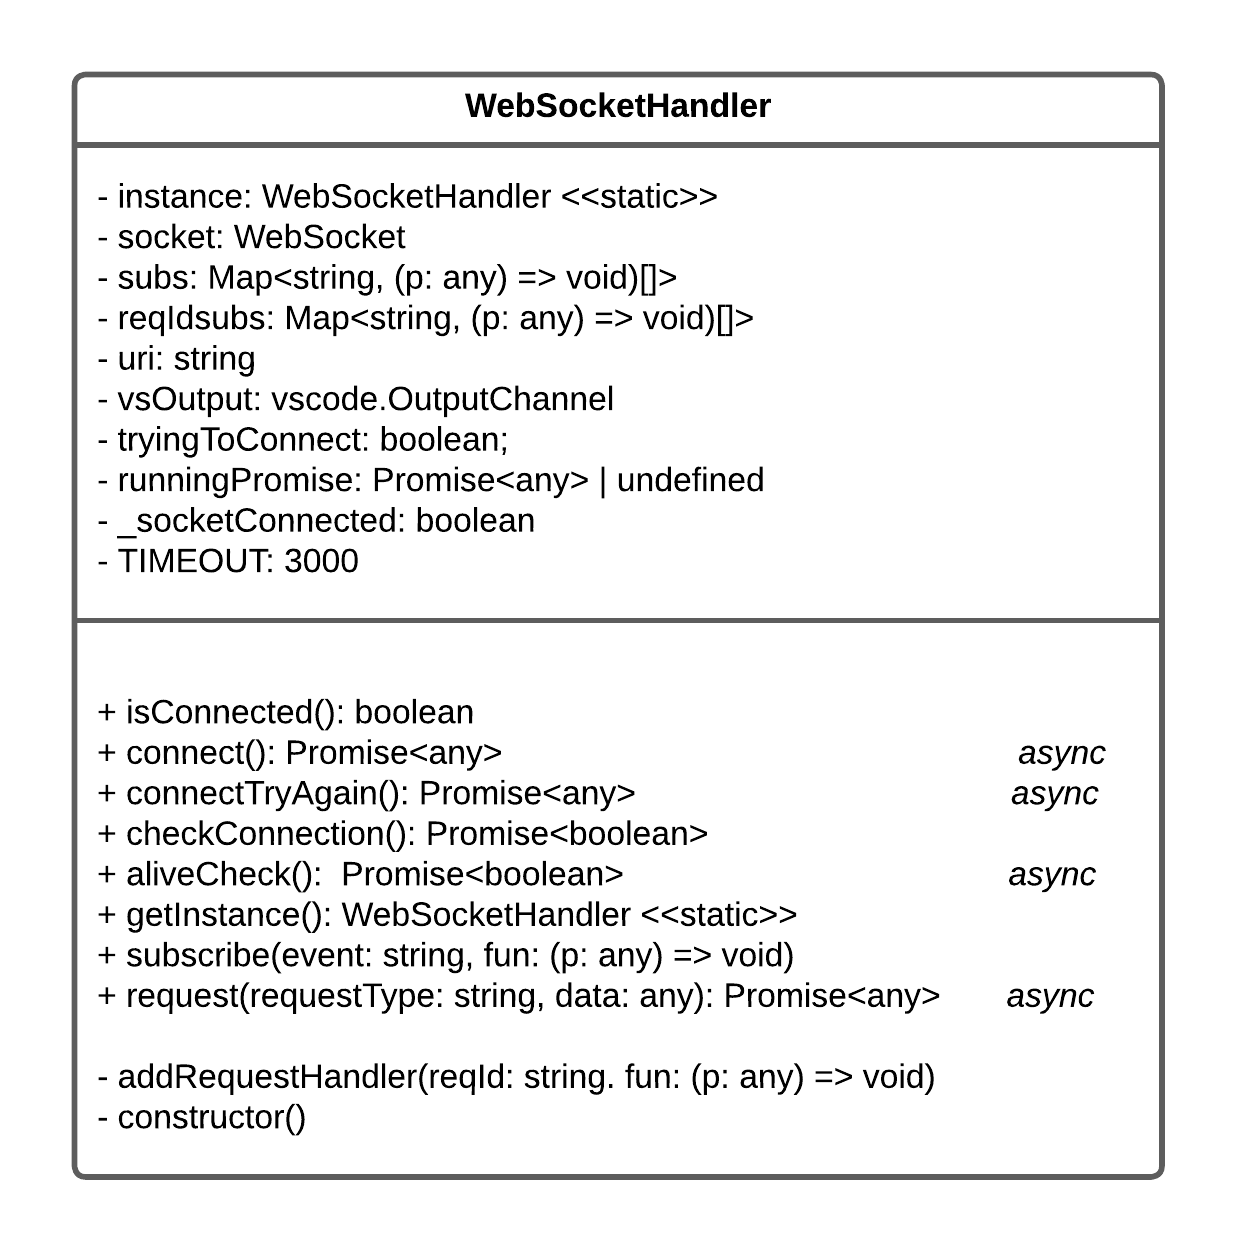
\includegraphics[width=0.8\linewidth]{images/wsDiagram.png}
  \caption{Komponensek viszonya egymáshóz}
  \label{fig:wsDiagram}
\end{figure}

Az osztály úgynevezett \textit{singleton} vagyis egyke tervezési mintát követ, tehát mindig csak egy példány lérezhet belőle. Ezt úgy lehet elérni, hogy a konstruktorját privát láthatóságúra állítjuk, így a példányosítása csakis osztályon belül lehetséges. A külső elérést a \lstinline{getInstance} metódus biztosítja, mely amennyiben már van egy példány visszadaj azt, amennyiben nincs létrehoz egyet.

\noindent Vegyük sorra az osztály publikus metódusait:

\begin{itemize}
    \item \lstinline{getInstance(): WebSocketHandler}: visszaadja az egyetlen példányt az osztályból 
    
    \item \lstinline{isConnected(): boolean}: megmondja, hogy van e aktív kapcsolat a Web Socketen keresztül
    
    \item \lstinline{connect(): Promise<any>}: ezzel kapcsolódhatunk a RefactorErl-hez Web Socketen keresztül. Helyes csatlakozés esetén az igíret (\textit{Promise}) feloldása esetén visszakapjuk az osztálypéldányt
    
    \item \lstinline{connectTryAgain(): Promise<any>}: annyiban más a \lstinline{connect()}-től, hogy megnézi azt, hogy van e kapcsolódási kísérlet folyamatban vagy sem, és folyamatason tájékoztatja a felhasználót a folyamatról. Lényegében amikor a felhasználó megnyomja a \textit{Try again} feliratú gombot a vezérlő pulton ez a metódus hívódik meg a háttérben.
    
    \item \lstinline{checkConnection(): Promise<boolean>}: leellenőrzi a Web Socket (WS) kapcsolatot a RefactorErl-el és erről tájékoztatja a felhasználót. Lényegében amikor a felhasználó megnyomja a \textit{Check connection} feliratú gombot a vezérlő pulton ez a metódus hívódik meg.
    
    \item \lstinline{aliveCheck(): Promise<boolean>}: ezzel a metódussal küldi el az \lstinline{alive} kérést a RefactorErl-nek.
    
    \item \lstinline{subscribe(event: string, fun: (p: any) => void: Promise<any>} feltudunk ezzel iratkozni egy esemény típusra, amit az első paraméterben tudunk megadni, a második paraméterében pedig az esemény lekezeléséhez használt függvényt kell megadni. \\ \\ A belső működése lényegében annyi, hogy egy szótár szerű objektumot tart karban aminek kulcsa az események típusai az értékek pedig az esemény kezelő függvények. Amikor egy bizonyos típusú esemény érkezik Web Socketen keresztül úgy ezen függvényeket sorban lefutatja, paraméterül adva az érkezett adatot.
    
    \item \lstinline{request(requestType: string, data: any): Promise<any>} ezen függvény segítségével tudunk kéréseket adni a RefactorErl felé. Az aszinkronitás kihasználása érdekében egy \textit{Promise} objektumot adunk vissza, ami tartalmazni fogja az eredményt ha elklészült. Paraméterül meg kell adnunk a lekérdezés típusát és az átküldendő adatot.

\end{itemize}

\subsubsection{\lstinline{dependencyGraphView.ts}}

A fájl két típust és egy osztályt definiál. Kezdjük a típusokkal először.



\\
\vspace{14pt}
\textbf{ViewState}
\\

Ez a típus reprezentál egy nézeti állapotot azálltal, hogy tárolja a gráf és az űrlap állapotát.

\begin{itemize}
    \item \lstinline{graph: GraphState | undefined}: a gráf állapota
    
    \item \lstinline{formState: DependencyGraphState | undefined: az űrlap állapota

\end{itemize}






\\
\vspace{14pt}
\textbf{GraphState}
\\

Ez a típus tárolja a gráf állapotát. Három lehetséges kombináció lehet:
\todo{bef}

\begin{itemize}
    \item \lstinline{graph: GraphState | undefined}: a gráf állapota
    
    \item \lstinline{formState: DependencyGraphState | undefined: az űrlap állapota

\end{itemize}
\todo{??}



\subsubsection{\lstinline{XX.d.ts}}


\todo{??}

\subsubsection{Kommunikáció a többi komponenssel}
\todo{??}
\section{Komponensek telepítőinek előállítása}

\todo{??}

\section{Teljes alkalmazás tesztelése}

Az automatikus tetszteket az egység tesztek szintjéig sikerült kivitelezni, de mivel két komplex rendszer összekötéséről van szó ezért rengeteg funkcionalitás csak manuálisan tesztelhető. A következőkben a manuális rendszer szintű tesztelés eseteit és eredményeit fogjuk áttekinteni

\subsection{Diagnosztikák tesztelése}

\noindent Tekintsük az alábbi teszt fájlt:

\lstset{caption=\lstinline{show.erl} teszt fájl, label=src:erlang} \label{mapConvertJson}
\begin{lstlisting}[language={erlang}] 
-module(show).
-export([safe_os_call/0, unsafe_os_call/1]).
-define(EXAMPLE_MACRO, 67).

safe_os_call() ->
    os:cmd("ls").

unsafe_os_call(A) ->
    os:cmd(A).
\end{lstlisting}

Ebben az esetben két diagnosztika aktív: \textit{nem használt makrók detektálása} és a \textit{nem biztonságos }

kép 

kép

console


(referl@fikoMac)26> ri:ls().                                        
{{ok,["/Users/fikorobert/Projects/ELS_Referl/els_dev/show.erl"]},{error,[]}}
ok
(referl@fikoMac)27> ri:q("mods[name=show].funs.unsecure_os_call").  
show:unsafe_os_call/1
    os:cmd(A)
ok
(referl@fikoMac)28> ri:q("mods[name=show].macros[not .references]").
show.erl
    EXAMPLE_MACRO
ok



\subsection{Változó Origin értékének kiszámításának tesztelése}

\subsection{Változó Reach értékének kiszámításának tesztelése}

\subsection{Függvény dinamikus hívásainak tesztelése}

\subsection{Modul függőségi gráfjának generálásának tesztelése}

\subsection{Függvény függőségi gráfjának generálásának tesztelése}

\subsection{Ürlap alapján gráf generálásának tesztelése}

\subsection{Vezérlőpult tesztelése}















